\subsection{Numerical Investigation of Propagating Modes in TEM Cells}\label{sec:modes_tem_cell}
\subsubsection{Mathematical derivation}
% Goal is to describe the modes in a TEM cell, including their cut-off frequencies. \cite{Kreindl_Bauernfeind_Weiss_Stockreitner_Kaltenbacher_2024} shows that these investigations are important. There are also modes propagating perpendicular to the intended propagation direction. Why are no waveguides used? Explain.

% In this paper, a VCSEL with a decoupling capacitor are modeled. It is visible, that the electric coupling dominates at an orientation of 90°. A local minimum is then visible. At 400\,MHz and upwards, inductive coupling becomes dominant, but only at 0° where it couples with the septum. It is possible, that a certain mode can propagate at a certain frequency, which influenced the result in this paper. 


Any electromagnetic field distribution in a waveguide can be represented by an infinite series of normal modes. \autoref{eqn:norm_power} shows that each mode is orthogonal to each other, with $\mathbf{e_n}^\pm$ and $\mathbf{h_n^\pm}$ being the function vectors of the electric and magnetic field in transverse direction \cite{Collin_2015}. A coupling between the modes only occurs due to geometric changes of the waveguide. Additionally, each mode carries unit power, shown by \autoref{eqn:unit_power}. Only the transverse fields are investigated in these Equations, because they carry power along the waveguide, opposed to the fields in the propagation direction.

\begin{align}
    \iint \mathbf{e_n^\pm}\times \mathbf{h_m^\pm}\mathrm{d}S\mathbf{n}&=0 \quad\text{if}\quad n\neq m
    \label{eqn:norm_power}\\
    \iint \mathbf{e_n^\pm}\times \mathbf{h_n^\pm}\mathrm{d}S\mathbf{n}&=1
    \label{eqn:unit_power}
\end{align}

Therefore, the radiated fields can be described by superposition of normals modes, as in \autoref{eqn:modal_superposition1} and \autoref{eqn:modal_superposition2}. These modes already consider the boundary conditions of the waveguide, therefore simplifying the calculations. The coefficients of these modes are straightforward to calculate, due to Lorentz Reciprocity Theorem, if the waveguide's walls are perfectly conducting. Also, if the dimensions of the waveguide is small enough, any higher order mode than the first TEM mode will be suppressed. 

\begin{align}
    \mathbf{E^\pm}&=\sum_na_n\mathbf{E_n^\pm}    \label{eqn:modal_superposition1}\\
    \mathbf{H^\pm}&=\sum_na_n\mathbf{H_n^\pm}    \label{eqn:modal_superposition2}
\end{align}

Suppose a current source $\mathbf{J_1}$ excites a waveguide (as is the case with the dipoles in the TEM cell). Normally, such a current source would be driven with external fields, but for the sake of the argument, they are ignored. Only $\mathbf{E}$ and $\mathbf{H}$ are considered, which are the fields radiated by $\mathbf{J_1}$. Additionally, $\mathbf{E_n^\pm}$ and $\mathbf{H_n^\pm}$ are the resulting transverse waveguide fields, with the signs indicating the direction of propagation. Take \autoref{eqn:lorentz_rec_theorem_int} and set $\mathbf{J_2}=\mathbf{M_1}=\mathbf{M_2}=0$. Now, only the current source $\mathbf{J_1}$ remains, and the \autoref{eqn:J1_propagating_waves} emerges. % Explain how certain surfaces do not to have be integrated, therefore rendering this equation very useful. Also, the expansion coefficients can be determined. Maybe do this calculation with a rectangular waveguide.

\begin{equation}
    \oiint _S (\mathbf{E_n^\pm}\times \mathbf{H}-\mathbf{E}\times \mathbf{H}_n^\pm)\cdot\mathrm{d}\mathbf{S}=\iiint \mathbf{J_1}\cdot\mathbf{E_n^\pm}\mathrm{d}V
    \label{eqn:J1_propagating_waves}
\end{equation}

In case of the TEM cell, it is desirable that only the TEM mode is propagating, and that the source is represented by a dipole. In the case of an electric dipole, therefore, the \autoref{eqn_dipole_tem_waves} arises. In this equation, the wave amplitudes $a$ and $b$ are given through the surface integral in the Lorentz Reciprocity theorem, with $a$ being the wave going to the left side, and $b$ to the other. The electric dipole moment $\mathbf{e_m}$ is given by the current $\mathbf{J}$ flowing through the infinitesimal wire. Note that only the electric field of TEM wave propagation is considered. In reality, more modes may propagate, for which the electric field must be replaced by the superposition of normal modes as in \autoref{eqn:modal_superposition1}. Additionally, to calculate the exact value of the electric field, a series of image sources as a Green's function may be applied.

\begin{equation}
\begin{pmatrix}a \\b\end{pmatrix} = -\frac{1}{2}\mathbf{m_e}\cdot \mathbf{E}^\pm
\label{eqn_dipole_tem_waves}
\end{equation}

\subsubsection{Modes in TEM cell}

A TEM cell is often used for EMC test specifications, as it enables the propagation of TEM waves, which resemble planar free-space waves. Additionally, it shields the waves from radiating to the sides, for which it has a clear advantage to a stripline \cite{809846}y
A simple rectangular waveguide cannot be used for this application. Assuming that a monochromatic wave traveling down the waveguide, the waves will propagate without dampening only at a certain angle of reflection on the perfectly conducting surface. A short mathematical proof can be shown here, using Maxwell's equation. It shows that the electric and magnetic fields in direction of propagation cannot both be zero. % Continue with some calculations, showing that TEM wave propagation is not possible?
\begin{align}
    \mathbf{E}&=(E_{0,x}\cdot\mathbf{e_x}+E_{0,y}\cdot\mathbf{e_y}+E_{0,z}\cdot\mathbf{e_z})\mathrm{e}^{\mathrm{i}(\omega t-kz)}\\
    \mathbf{H}&=(H_{0,x}\cdot\mathbf{e_x}+H_{0,y}\cdot\mathbf{e_y}+H_{0,z}\cdot\mathbf{e_z})\mathrm{e}^{\mathrm{i}(\omega t-kz)}\\
    \nabla \times \mathbf{E} &=\begin{pmatrix}\frac{\mathrm{d}}{\mathrm{d}y}E_z-\mathrm{i}kE_y \\\mathrm{i}kE_x-\frac{\mathrm{d}}{\mathrm{d}x}E_z \\\frac{\mathrm{d}}{\mathrm{d}x}E_y-\frac{\mathrm{d}}{\mathrm{d}y}E_x\end{pmatrix}=\begin{pmatrix} -\mathrm{i}\omega B_x\\-\mathrm{i}\omega B_y\\ -\mathrm{i}\omega B_z \end{pmatrix}\\
    \nabla \times \mathbf{B} &=\begin{pmatrix}\frac{\mathrm{d}}{\mathrm{d}y}B_z-\mathrm{i}kB_y \\\mathrm{i}kB_x-\frac{\mathrm{d}}{\mathrm{d}x}B_z \\\frac{\mathrm{d}}{\mathrm{d}x}B_y-\frac{\mathrm{d}}{\mathrm{d}y}B_x\end{pmatrix}=\begin{pmatrix} \frac{\mathrm{i}\omega}{\mu\epsilon} E_x\\\frac{\mathrm{i}\omega}{\mu\epsilon} E_y\\ \frac{\mathrm{i}\omega}{\mu\epsilon} E_z \end{pmatrix}
\end{align}

If $E_z$ and $B_z$, the fields in direction of propagation, were both zero, then the change of the transverse fields would be constantly zero, and because of the boundary conditions, all transverse fields would be zero. \autoref{eqn:rect_waveguide_gauss} shows Gauss' law and \autoref{eqn:rect_waveguide_faraday} Faraday's law if $E_z=B_z=0$, from which the unchanging transverse electric field can be derived. A TEM cell solves this problem, by having a gap between the septum and the side walls. This makes it essentially to two rectangular waveguides with apertures on the sides, which enable perturbation between them. Since the boundary conditions of the Laplace equation now changed, due to the gaps, the electric and magnetic fields do not have to be constantly zero across the transverse plane. The Green's function may be calculated of the new construction, now considering the boundary conditions at the gaps, which must be the same for both waveguides (to prevent discontinuities) \cite{Tippet_Chang_Crawford_1976}.

The TEM cell used in the simulation has a width of $a=200\,\mathrm{mm}$ and a height $b=100\,\mathrm{mm}$. The cutoff frequencies of TE\textsubscript{m,2n} and TM\textsubscript{m,2n} modes in a TEM cell may be approximated by \autoref{eqn:cutoff_frequency_rect_waveguide}, which is the same formula for rectangular waveguides. This works because a thin conducting layer, as the septum is, does not influence these modes \cite{Weil_Gruner_1984}. Consequently, the cutoff frequency of the first TE\textsubscript{01} mode must be around 750\,MHz. This proposition is checked with a modal simulation in Ansys HFSS, its resulting S-parameters are shown in \autoref{fig:te01_tem_modes_propagation}. The green line shows the S\textsubscript{12}-parameter over the frequency of the TEM mode, while the red line demonstrates S\textsubscript{12}-parameter of the TE\textsubscript{01} mode. At a frequency of 751\,MHz, the mode propagates without attenuation, hence there is the cutoff frequency. The simulated result comes very close to the analytically determined one.

\begin{equation}
    f_c = \frac{c}{2} \sqrt{\left(\frac{m}{a}\right)^2 + \left(\frac{n}{b}\right)^2}
    \label{eqn:cutoff_frequency_rect_waveguide}
\end{equation}

\begin{itemize}
  \item \( f_c \): cutoff frequency of the mode \(\text{T}_{mn}\)
  \item \( c \): speed of light in the medium (approximately \(3 \times 10^8 \, \text{m/s}\) in air)
  \item \( a \): wider dimension (broad wall) of the rectangular waveguide (meters)
  \item \( b \): narrower dimension (narrow wall) of the rectangular waveguide (meters)
  \item \( m \): mode index in the \(a\)-direction (integer, \(m \geq 0\))
  \item \( n \): mode index in the \(b\)-direction (integer, \(n \geq 0\))
\end{itemize}

\begin{figure}[h]
    \centering
    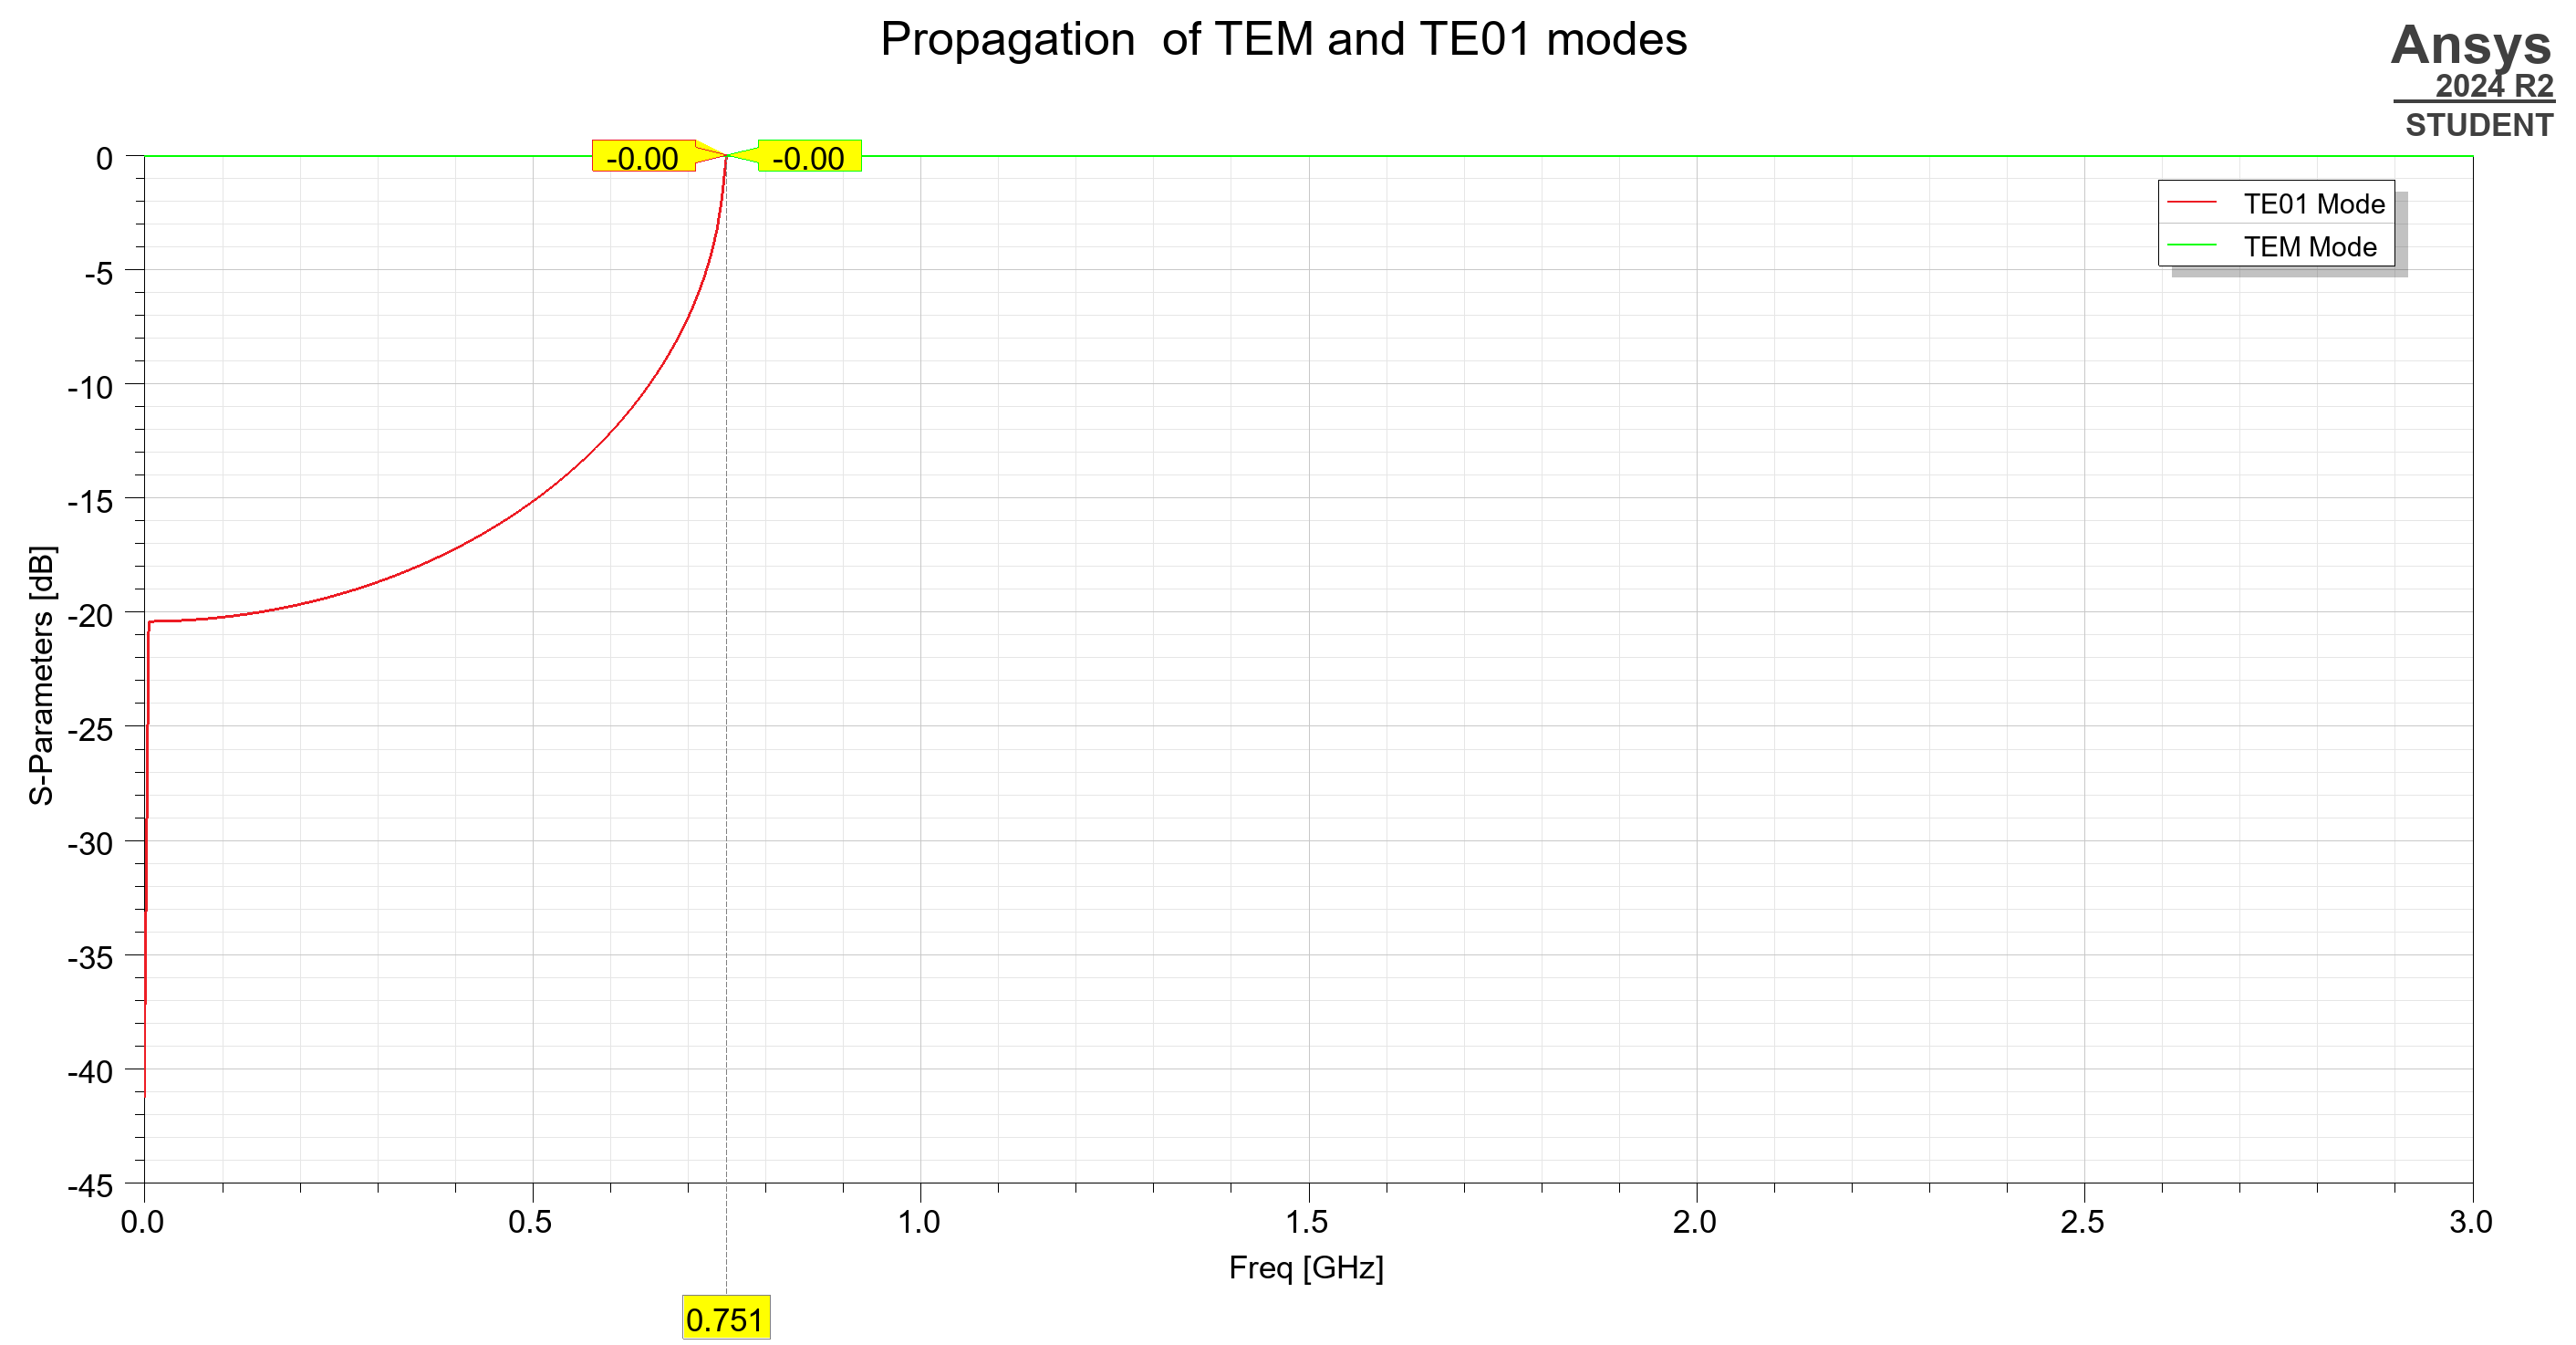
\includegraphics[width=1\linewidth]{Documentation//content//10_theory//img/te01_tem_modes_propagation.png}
    \caption{Propagation of TEM and TE\textsubscript{01} modes in TEM cell}
    \label{fig:te01_tem_modes_propagation}
\end{figure}


\begin{align}
    \frac{\mathrm{d}}{\mathrm{d}x}E_x+\frac{\mathrm{d}}{\mathrm{d}y}E_y&=0\quad\text{Gauss' law}\label{eqn:rect_waveguide_gauss}\\
    \frac{\mathrm{d}}{\mathrm{d}y}E_x-\frac{\mathrm{d}}{\mathrm{d}x}E_y&=0\quad\text{Faraday's law}\label{eqn:rect_waveguide_faraday}
\end{align}


The TEM cell does not only support TEM modes, above their cut-off frequency TE and TM modes begin to propagate. Because the TEM cell is a high-Q cavity, those cut-off frequencies are sharply defined frequencies. However, some modes might begin to propagate below their cut-off frequency due to imperfections, change in materials or finite conductivity of the conducting plates \cite{10791592}. A change in material, for example, demands the electric and magnetic field to have a component in the direction of propagation at the discontinuity. A paper by Wilson and Ma present analytical approximations to determine these frequencies \cite{Wilson_Ma_1986}.  There is a long list for the several first few corner frequencies of the first modes. Additionally, a paper by Koch, Groh and Garbe determines the resonance frequencies of the first TE modes analytically \cite{10791592}.

\begin{figure}[h]
    \centering
    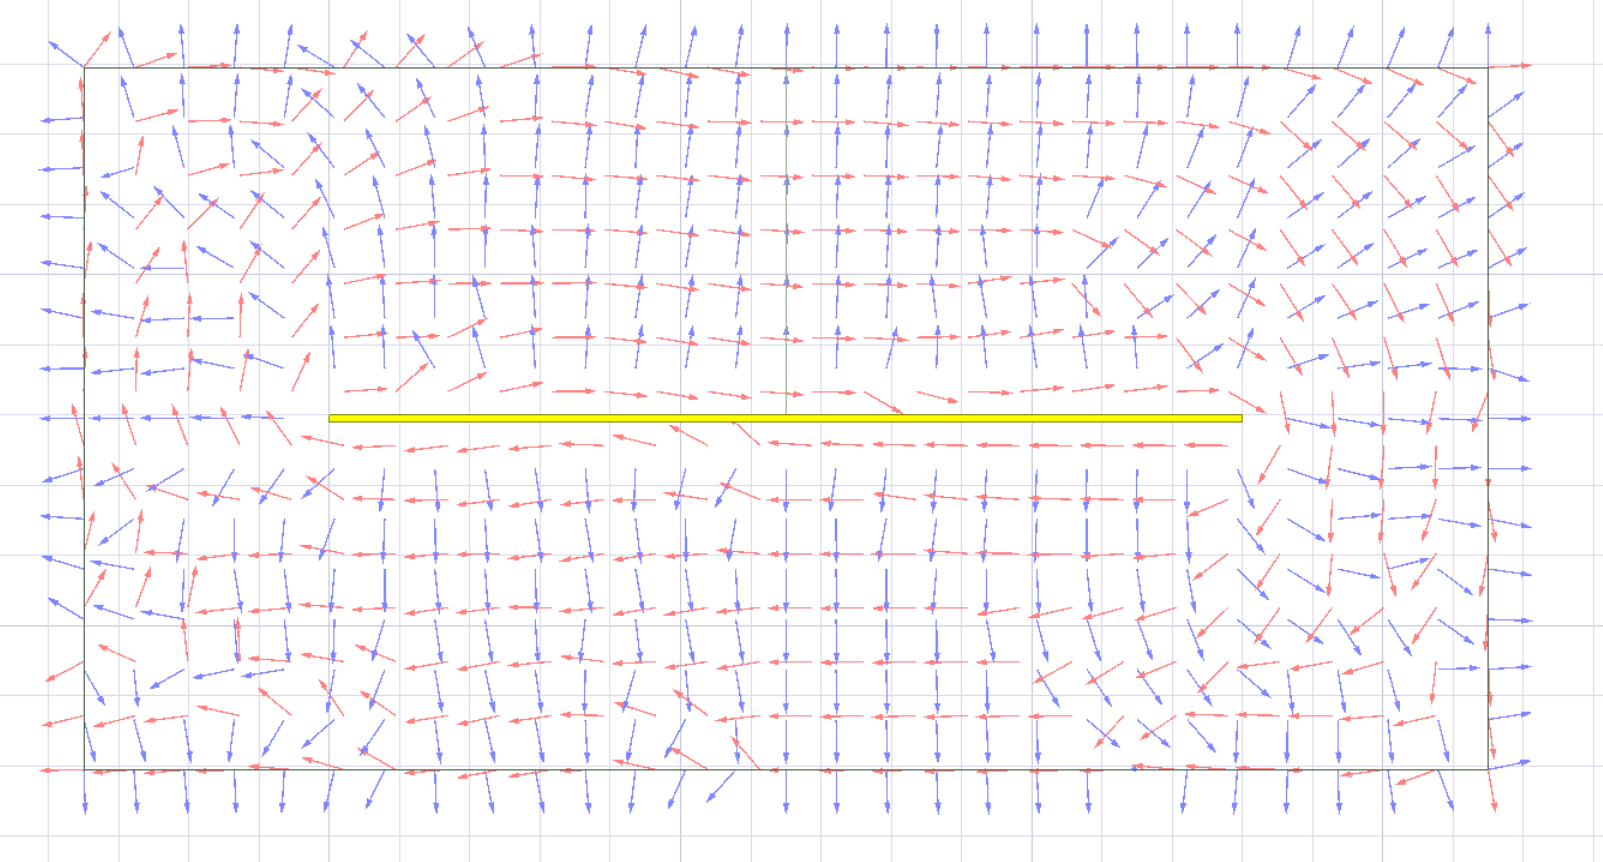
\includegraphics[width=0.5\linewidth]{images/tem_mode.png}
    \caption{TEM Mode}
    \label{fig:tem_mode}
\end{figure}
%(My TEM cell is too short to have more modes than this) Investigation of more modes would be interesting

The first mode after the TEM mode is the TE\textsubscript{01}, depicted in \autoref{te01_mode_temcell}. Note that the index of the modes indicate the spatial variation of the fields, as in a cylindrical waveguide. In many papers, as in \cite{Tippet_Chang_Crawford_1976}, the Green's function and the modes of the TEM cell are treated like in a cylindrical waveguide. The first index indicates variation in azimuthal direction, the second in radial direction.

\begin{figure}[h]
    \centering
    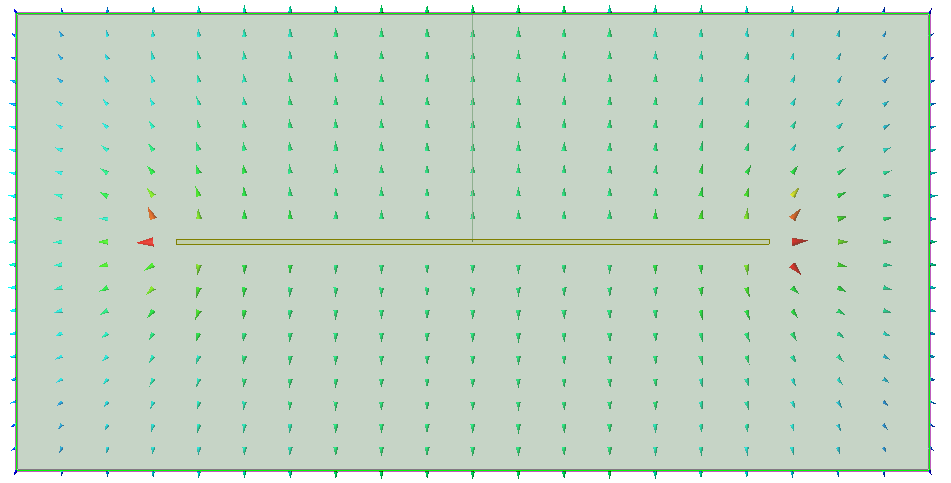
\includegraphics[width=0.5\linewidth]{Documentation//content//10_theory//img/te01_mode_temcell.png}
    \caption{TE\textsubscript{01} mode of TEM cell}
    \label{fig:te01_mode_temcell}
\end{figure}

\begin{figure}[h]
    \centering
    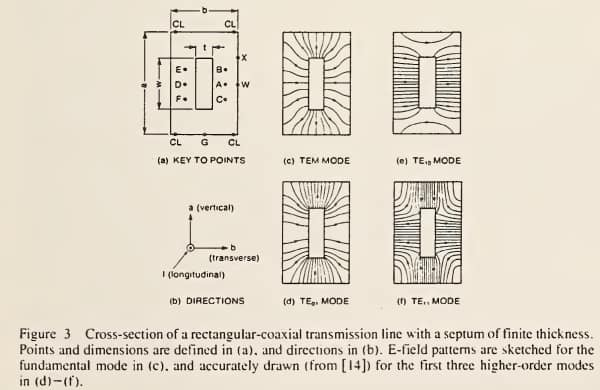
\includegraphics[width=0.5\linewidth]{Documentation//content//10_theory//img/delete_after.png}
    \caption{NUR FÜR REFERENZ}
    \label{fig:placeholder}
\end{figure}

